\section{Approach}
\label{sec:approach}

\begin{figure}
	\begin{center}
		%\begin{framed}
		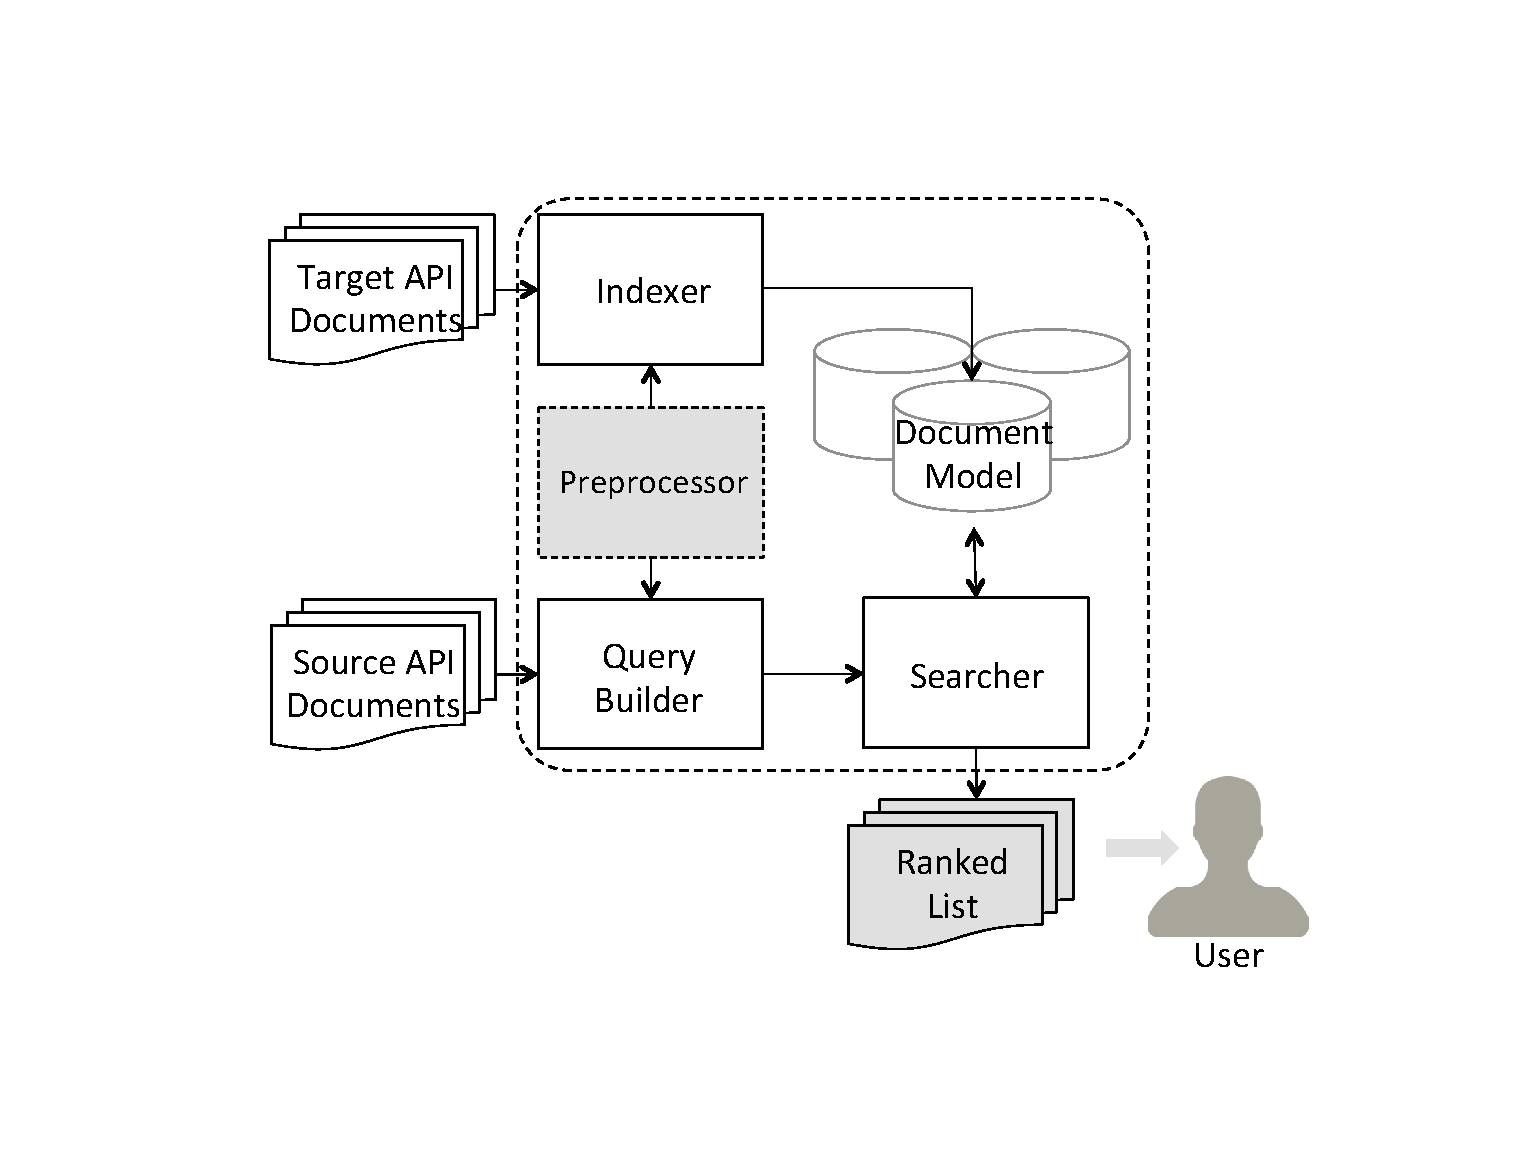
\includegraphics[scale=0.45,clip=true, trim=100pt 80pt 100pt 100pt]{ApproahOverview.eps}
		%\end{framed}
		\caption{\label{fig:approachOverview} Overview of \tool\ approach}
	\end{center}
\end{figure}




We first preprocess the API documents

In particular we extract the fields listed in Table~\ref{tab:extractedFields} fields from API documents

\begin{table}
	\begin{center}
		\caption{Extracted Fields}
		\begin{small}
			\begin{tabular}{rll}
				\topline
				\headcol 	S No. 	& Name	& Description \\
				\midline 
				
				\rowpln 1	& Type Name				& Enclosing class/interface name of the method \\
				\rowcol 2	& Package Name			& Package name of the enclosing class\\
				\rowpln 3	& Method Name			& Name of the method \\
				\rowcol 4	& Method Modifiers		& Access modifiers of the method \\
				\rowpln 5	& Exceptions Thrown		& Name of the exceptions thrown by the method \\
				\rowcol 6	& Parameters			& Name and type information of parameters \\
				\rowpln 7	& Class Description		& Description of enclosing type \\
				\rowcol 8	& Method Description	& Description of the method \\			
				\bottomline
				%----------------- END TABLE DATA ------------------------ 
			\end{tabular}
			\label{tab:extractedFields}
		\end{small}
		
	\end{center}
\end{table}

We perform the following pre-processing

\begin{enumerate}
	\item \textbf{Lowercase} Convert the text to lowercase
	\item \textbf{Split Camelcase} Split the camelcase notation of the class name and method name
	\item \textbf{Split package Notation} Split the package notation
	\item \textbf{Remove href and other javadoc identifiers} remove the \CodeIn{@Code, @link}... like \CodeIn{JavaDoc} identifers
\end{enumerate}


First we parse the API documents of source and target API library and store it in intermediate representation for analysis. In particular, we extract class, interface and corresponding method descriptions from API documents. Second, we then create a term vector representation of each class description and method descriptions. Vector space model or term vector model is an algebraic model for representing text documents (and any objects, in general) as vectors of identifiers, such as, for example, index terms. In our case, each word is considered as a term barring the stop words such as (a, the, and ...). 

Finally we use the term vector representation of a method description in a source API to query term vector representation of the the method description in target API. The results are ranked based on the Term Frequency-Inverse Document Frequency (TF-IDF) measure. TF-IDF is a numerical statistic which reflects how important a word is to a document in a collection or corpus. It is often used as a weighting factor in information retrieval and text mining.


We next build indexes 

Lucene Indexes 

using Standard English Analyzer

following fields:

Class Base Name Camel Case Split

Class Description

Method base Name Camel Case Split

Method Description


Query formulation:

heuristics 1 : first two sentences are provide a reasonable approximation of the most important keywords of an method

heuristics 2 : first paragraph provides a reasonable approximation of the most important keywords of a class.

\begin{figure}
	\begin{framed}	
		\textbf{Class Name}: \CodeIn{java util iter}\\
		\textbf{Class Description}: \CodeIn{iter over collect iter take enumer java collect framework}\\
		\textbf{Method Name}$^*$: \CodeIn{ha next}\\
		\textbf{Method Description}: \CodeIn{return true iter ha more element other word return true next would return elementrather than throw except}\\ \\
		$^*$ Names are Camel-case split
	\end{framed}
	\caption{Query}
	\label{fig:hasNextJavaQuery}
\end{figure}


\begin{figure}
	\begin{framed}
		{\LARGE hasNext}\\
		\CodeIn{boolean hasNext()}\\
		Returns \CodeIn{true} if the iteration has more elements. (In other words, returns true if \CodeIn{next()} would return an element rather than throwing an exception.)\\
		\textbf{Returns}:\\
		\CodeIn{true} if the iteration has more elements
	\end{framed}
	\caption{hasNext method of Iterator}
	\label{fig:hasNextJavadoc}
\end{figure}
